% This file was created with tikzplotlib v0.10.1.
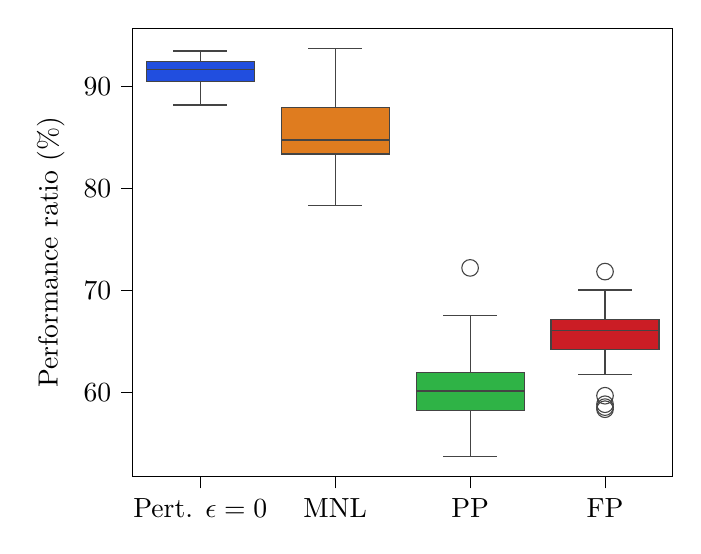
\begin{tikzpicture}

\definecolor{chocolate22312431}{RGB}{223,124,31}
\definecolor{darkgray176}{RGB}{176,176,176}
\definecolor{darkslategray68}{RGB}{68,68,68}
\definecolor{firebrick2032937}{RGB}{203,29,37}
\definecolor{limegreen4717970}{RGB}{47,179,70}
\definecolor{royalblue3378223}{RGB}{33,78,223}

\begin{axis}[
tick align=outside,
tick pos=left,
x grid style={darkgray176},
xmin=-0.5, xmax=3.5,
xtick style={color=black},
xtick={0,1,2,3},
xticklabels={Pert. \(\displaystyle \epsilon=0\),MNL,PP,FP},
y grid style={darkgray176},
ylabel={Performance ratio (\%)},
ymin=51.7327333589047, ymax=95.705322244542,
ytick style={color=black},
ytick={50,60,70,80,90,100},
yticklabels={
  \(\displaystyle {50}\),
  \(\displaystyle {60}\),
  \(\displaystyle {70}\),
  \(\displaystyle {80}\),
  \(\displaystyle {90}\),
  \(\displaystyle {100}\)
}
]
\path [draw=darkslategray68, fill=royalblue3378223]
(axis cs:-0.4,90.450776630759)
--(axis cs:0.4,90.450776630759)
--(axis cs:0.4,92.4829044807425)
--(axis cs:-0.4,92.4829044807425)
--(axis cs:-0.4,90.450776630759)
--cycle;
\addplot [darkslategray68]
table {%
0 90.450776630759
0 88.1720209517941
};
\addplot [darkslategray68]
table {%
0 92.4829044807425
0 93.4733527349877
};
\addplot [darkslategray68]
table {%
-0.2 88.1720209517941
0.2 88.1720209517941
};
\addplot [darkslategray68]
table {%
-0.2 93.4733527349877
0.2 93.4733527349877
};
\path [draw=darkslategray68, fill=chocolate22312431]
(axis cs:0.6,83.370784409605)
--(axis cs:1.4,83.370784409605)
--(axis cs:1.4,87.9421723344371)
--(axis cs:0.6,87.9421723344371)
--(axis cs:0.6,83.370784409605)
--cycle;
\addplot [darkslategray68]
table {%
1 83.370784409605
1 78.3111257451702
};
\addplot [darkslategray68]
table {%
1 87.9421723344371
1 93.7065682042857
};
\addplot [darkslategray68]
table {%
0.8 78.3111257451702
1.2 78.3111257451702
};
\addplot [darkslategray68]
table {%
0.8 93.7065682042857
1.2 93.7065682042857
};
\path [draw=darkslategray68, fill=limegreen4717970]
(axis cs:1.6,58.1983222317439)
--(axis cs:2.4,58.1983222317439)
--(axis cs:2.4,61.9153945878929)
--(axis cs:1.6,61.9153945878929)
--(axis cs:1.6,58.1983222317439)
--cycle;
\addplot [darkslategray68]
table {%
2 58.1983222317439
2 53.731487399161
};
\addplot [darkslategray68]
table {%
2 61.9153945878929
2 67.4878542291351
};
\addplot [darkslategray68]
table {%
1.8 53.731487399161
2.2 53.731487399161
};
\addplot [darkslategray68]
table {%
1.8 67.4878542291351
2.2 67.4878542291351
};
\addplot [black, mark=o, mark size=3, mark options={solid,fill opacity=0,draw=darkslategray68}, only marks]
table {%
2 72.1973492131034
};
\path [draw=darkslategray68, fill=firebrick2032937]
(axis cs:2.6,64.2016330129495)
--(axis cs:3.4,64.2016330129495)
--(axis cs:3.4,67.1314118422844)
--(axis cs:2.6,67.1314118422844)
--(axis cs:2.6,64.2016330129495)
--cycle;
\addplot [darkslategray68]
table {%
3 64.2016330129495
3 61.7273700318582
};
\addplot [darkslategray68]
table {%
3 67.1314118422844
3 70.0340493056789
};
\addplot [darkslategray68]
table {%
2.8 61.7273700318582
3.2 61.7273700318582
};
\addplot [darkslategray68]
table {%
2.8 70.0340493056789
3.2 70.0340493056789
};
\addplot [black, mark=o, mark size=3, mark options={solid,fill opacity=0,draw=darkslategray68}, only marks]
table {%
3 58.542062452697
3 59.6589528057897
3 58.8263570050731
3 58.3384168869763
3 71.833140233908
};
\addplot [darkslategray68]
table {%
-0.4 91.6217044635638
0.4 91.6217044635638
};
\addplot [darkslategray68]
table {%
0.6 84.7378846675944
1.4 84.7378846675944
};
\addplot [darkslategray68]
table {%
1.6 60.118417064117
2.4 60.118417064117
};
\addplot [darkslategray68]
table {%
2.6 66.0223193072873
3.4 66.0223193072873
};
\draw (axis cs:0,40.7395861374954) node[
  scale=0.75,
  anchor=base,
  text=black,
  rotate=0.0
]{\bfseries 91.34};
\draw (axis cs:1,40.7395861374954) node[
  scale=0.75,
  anchor=base,
  text=black,
  rotate=0.0
]{\bfseries 85.39};
\draw (axis cs:2,40.7395861374954) node[
  scale=0.75,
  anchor=base,
  text=black,
  rotate=0.0
]{\bfseries 60.33};
\draw (axis cs:3,40.7395861374954) node[
  scale=0.75,
  anchor=base,
  text=black,
  rotate=0.0
]{\bfseries 65.20};
\draw (axis cs:-1,41.1793120263518) node[
  scale=0.75,
  text=black,
  rotate=0.0
]{\bfseries \textbf{Average:}};
\end{axis}

\end{tikzpicture}
